\documentclass{beamer}
\usetheme{Warsaw}
%\setbeameroption{show only notes}
\usefonttheme[onlylarge]{structurebold}
\setbeamerfont*{frametitle}{size=\normalsize,series=\bfseries}
\setbeamertemplate{navigation symbols}{}
\usepackage[english]{babel}
\usepackage{setspace}
\usepackage[latin1]{inputenc}
\usepackage{times}
\usepackage[T1]{fontenc}
\usepackage{tikz}
\bibliographystyle{acm}
\usetikzlibrary{arrows}
\usepackage{soul}
\usepackage{chronosys}
\usepackage{color}
\tikzstyle{block}=[draw opacity=0.3,line width=1.4cm]

\title{Linked Open Data - the value-add to a postcard collection}
%\subtitle{or, representing an untidy world on paper}
\author[Warren and Farnel, Farnel and Warren]
{
 Sharon Farnel\inst{2} \and Maharsh Patel\inst{2} \and   Rob Warren\inst{1}
}
\institute[]
{
  \inst{1}%
  {\small rwarren@math.carleton.ca} - @muninn\_project \\
Carleton University \\
\inst{2}
{\small sharon.farnel@ualberta.ca}\\
University of Alberta 
}
\usebackgroundtemplate{%
\tikz[overlay,remember picture] \node[opacity=0.15, at=(current page.center)]
{
 \centering
 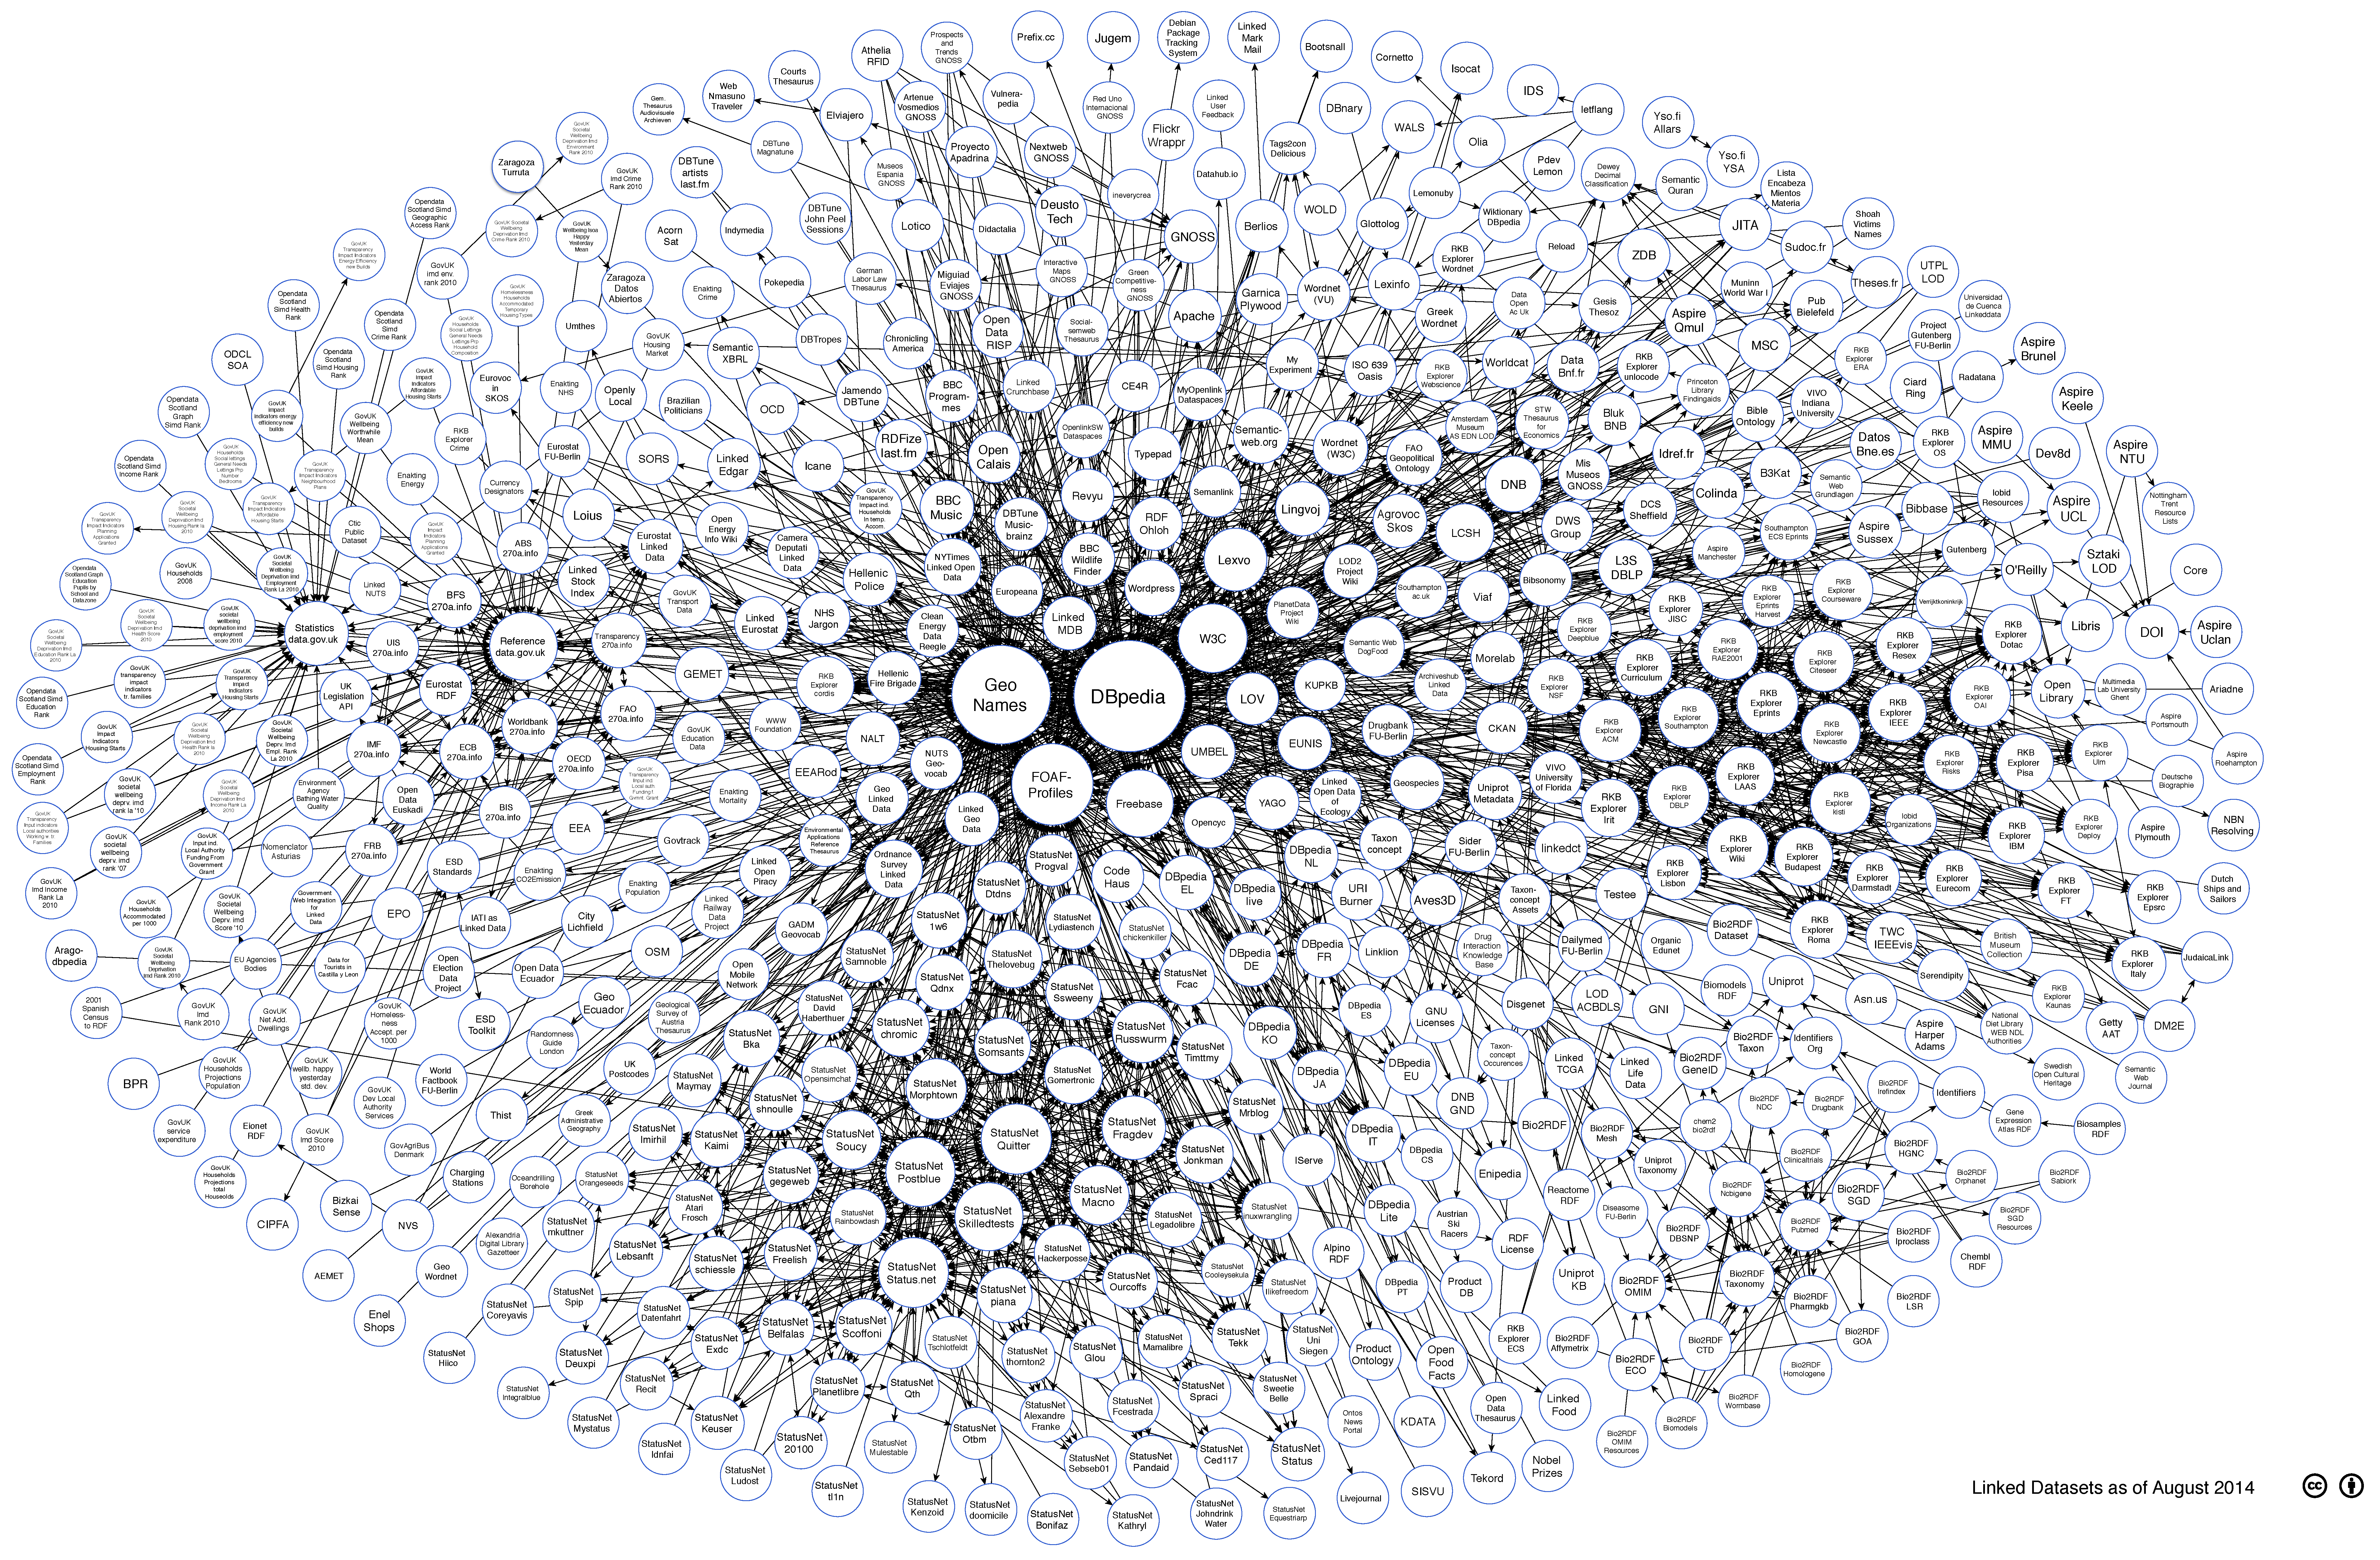
\includegraphics[width=0.98\paperwidth]{figures/lod-cloud}};
}
\date[Access 2017]{September, 2017}
%\includegraphics[height=0.5in]{figures/institutelogo}}
%\usebackgroundtemplate{%
%\tikz[overlay] \node[opacity=0.15, at=(current page.center)]
%{
% \centering
% 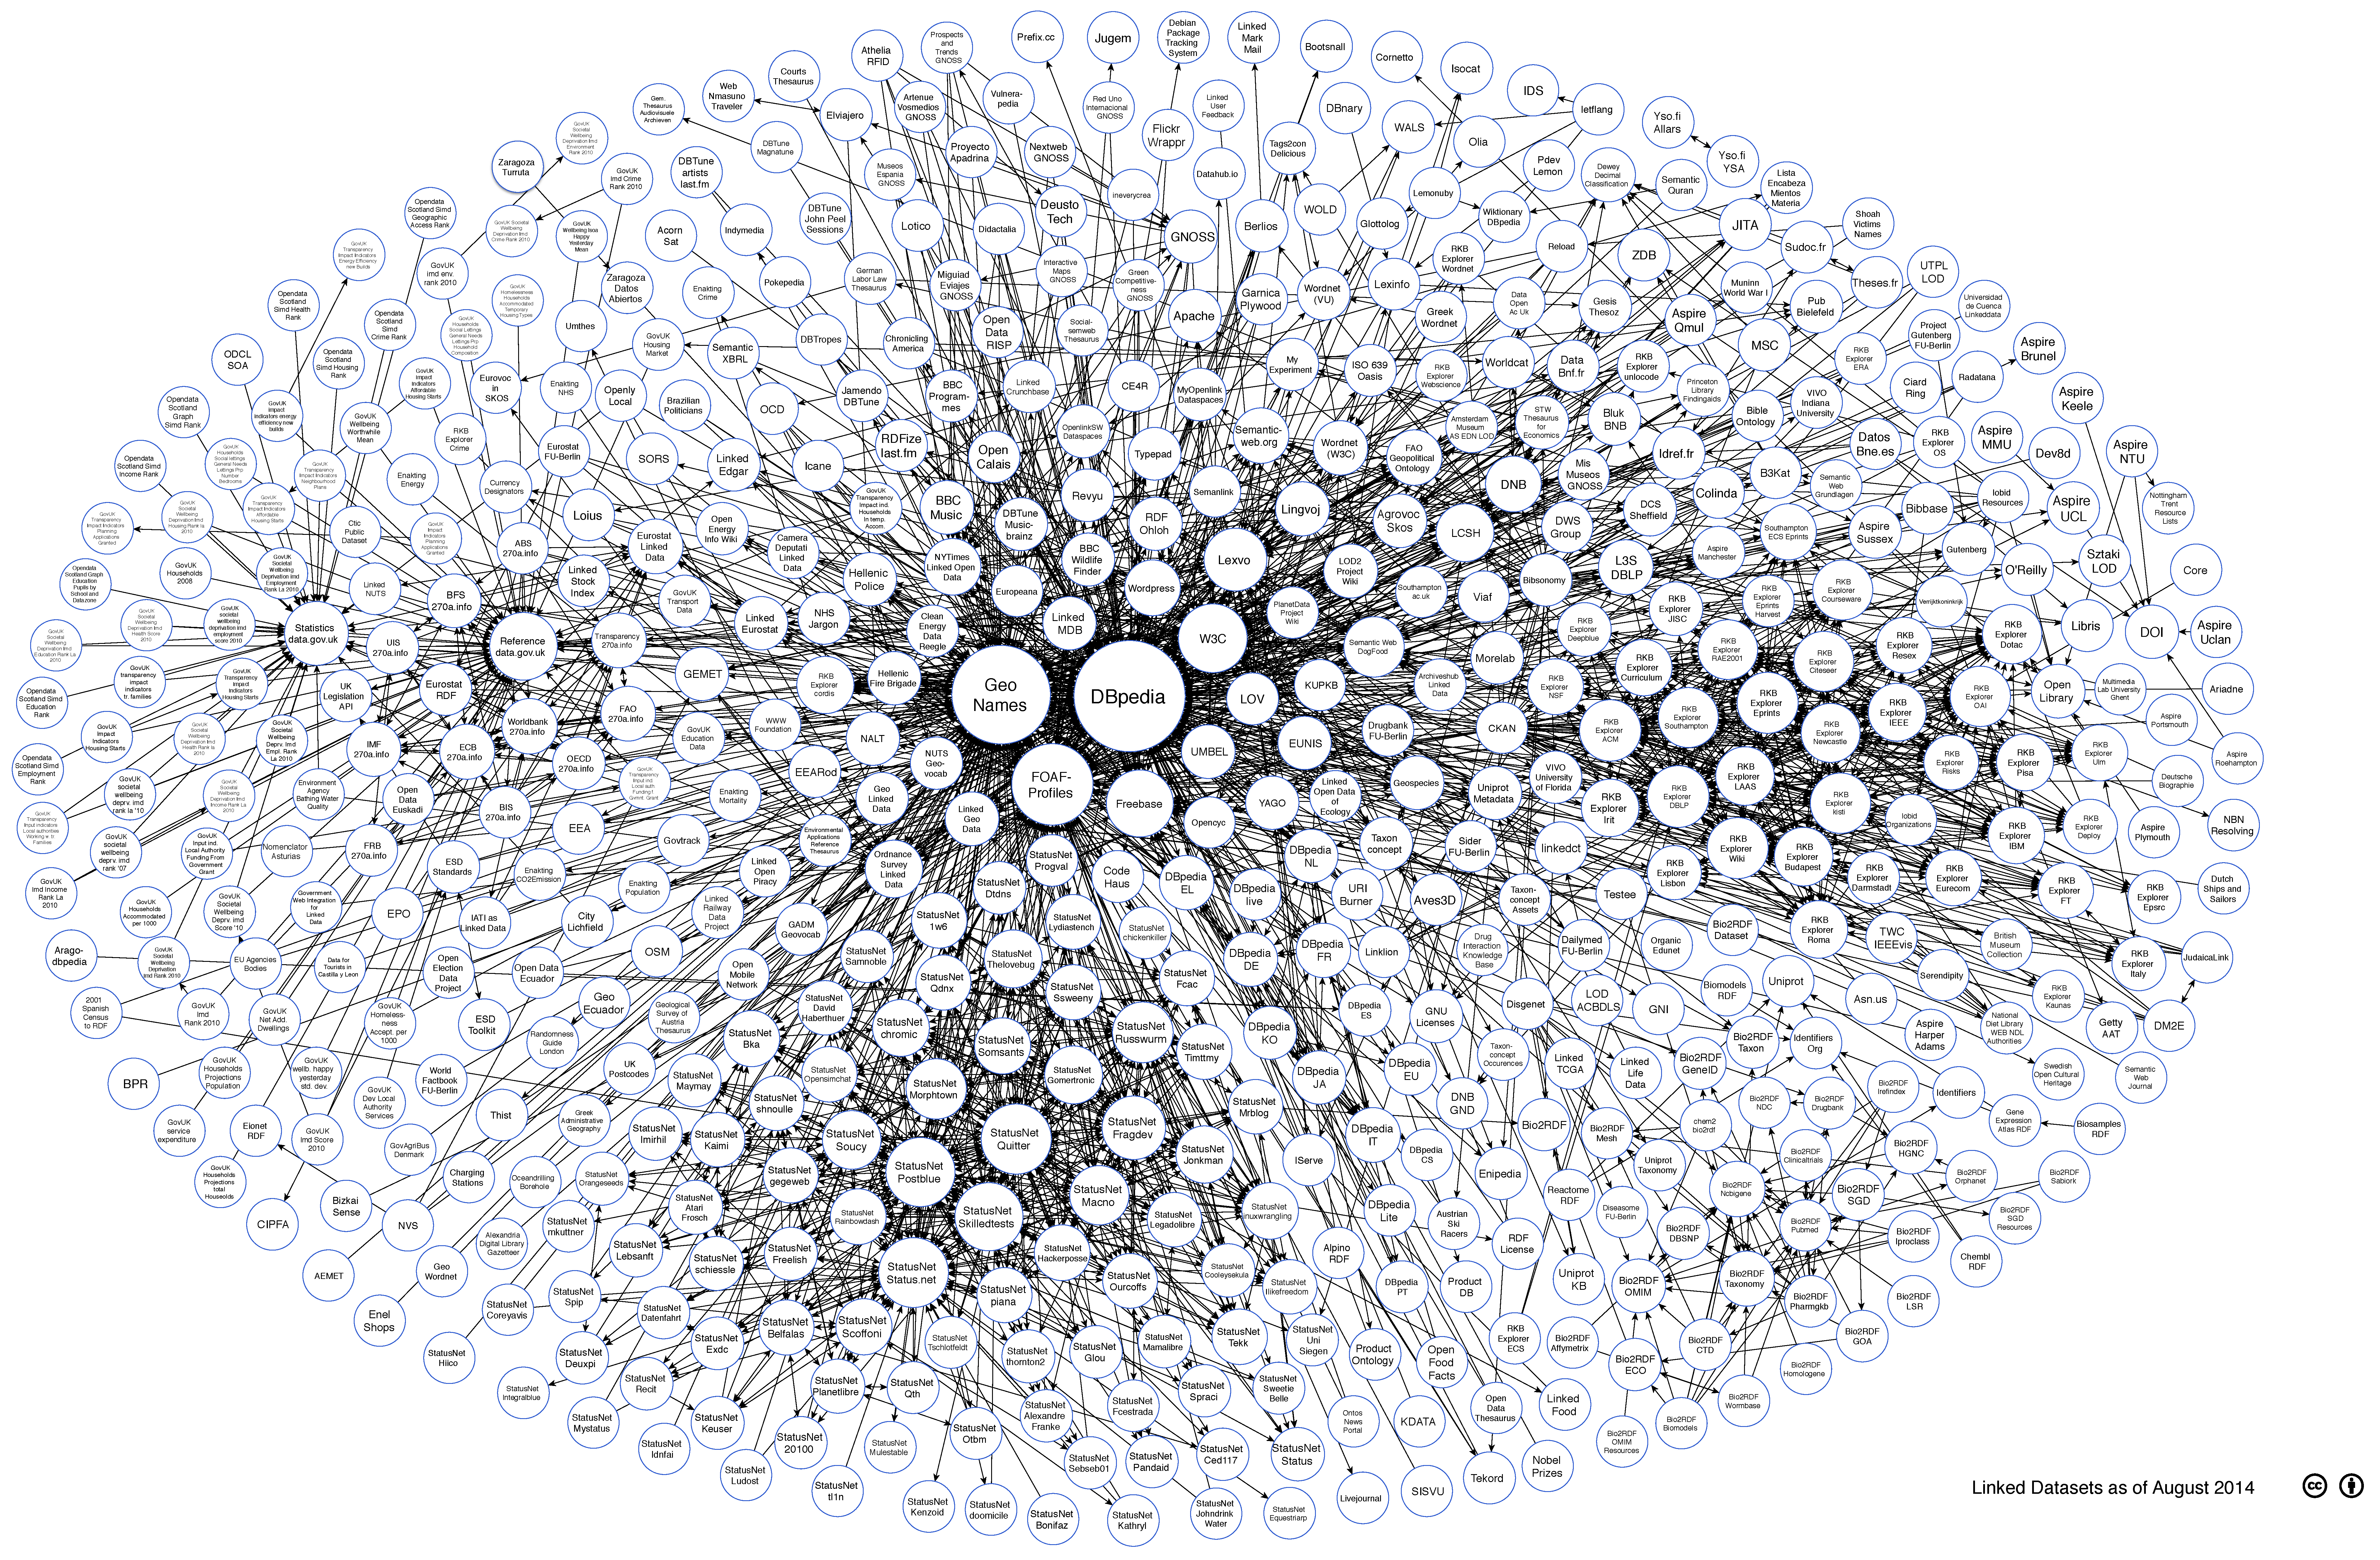
\includegraphics[width=0.95\paperwidth]{figures/lod-cloud}};
%}
%\date[searchisover.org]{The Search Is Over! - Exploring Cultural Collections with Visualization - DL2015}
% The main document
\useoutertheme{infolines}
%\makeatletter
%    \newenvironment{withoutheadline}{
%
%        \setbeamertemplate{headline}[default]
%        \def\beamer@entrycode{\vspace*{-\headheight}}
%  }{}
%kx\makeatother
\begin{document}


\begin{frame}
  \titlepage
\end{frame}

%\begin{withoutheadline}
\usebackgroundtemplate{}
\frame{\tableofcontents}
%\section{Introduction}

%   \begin{frame}
%        \frametitle{Presentation Outline}
%        \tableofcontents[currentsection,currentsubsection]
%   \end{frame}

%        \frametitle{Presentation Outline}
%        \tableofcontents[currentsection,currentsubsection]
%   \end{frame}

\section{Introduction}

\section{Conclusion}

\begin{frame}
communications and the arts - music / communication et les arts - musique (umi : 0413)
\end{frame}

%
% How 
% MUN_4971_Theses_for_CLDI_linked.mrc: 11860/12541 found correctly
%qs_thesis.mrc: 6918/20925
%CLDI_LAC_bib_file.mrc: 225/823 found
%U_Montreal_100_BibliographicRecords_from_IR.mrc: 228/1366
%U_Montreal_100_BibliographicRecords_from_ILS.mrc: 73/301
%
% 90% closeness. Even with this percentage I am getting errors where it converts things like "Historical Drama" to "Historical Trauma". I
%



\begin{frame}
\begin{alertblock}{}
Everything and the ktichen sink
\end{alertblock}
\end{frame}

\begin{frame}
\begin{alertblock}{}
peopel and machiens are no physici; need ontology.
\end{alertblock}
\end{frame}

\begin{frame}
\begin{block}{}
\begin{itemize}
\item Sparql server.
\item Keywork searchable.
\item cross linked to authorities.
\item RIS/Bibtex exports.
\item Ontology published.
\end{itemize}
\end{block}
\end{frame}

\begin{frame}
\begin{block}{Maintenance}
\begin{itemize}
\item Direct output to github tickets
\item Twitter uploade acconutments
\item Twitter thesis of the day.
\end{itemize}
\end{block}
\end{frame}




\begin{frame}
\begin{block}{Why?}
Merge finanical data with the thesis data. Comes out to xB\$ in sunk costs, let's get value out of it.
\end{block}
\end{frame}


\begin{frame}
\begin{block}{Trends}
Who gets the most PhD's per capita?
\end{block}
\end{frame}

\begin{frame}
\begin{block}{Trends}
What were the most popular keywords in the list.
\end{block}
\end{frame}


\begin{frame}
\begin{block}{Lessons Learned, Next Steps}
\begin{itemize}
\item ....
\end{itemize}
\end{block}
\begin{alertblock}{}
Code and scripts at: \url{https://github.com/rwarren2/CanLink.git}
\end{alertblock}
\end{frame}

%\end{withoutheadline}

\end{document}

